\section{Hypothesis} \label{sec:hypothesis}
    
  {\bf $H_{0}$: Human properties have no influence in users choice of graphical passwords} 

  {\bf $H_{1}$: Users choice of graphical passwords are influenced by the human properties of the user}

  The tested hypothesis is referred to as the null hypothesis (abbreviated $H_{0}$). We start with the assumption that the null hypothesis is true; human properties have no influence on users choice of graphical passwords. Along with $H_{0}$ it is stated an alternative hypothesis (abbreviated $H_{1}$). The alternative hypothesis states that users choice in graphical passwords is influenced by the human properties of the user. If the null hypothesis is rejected, we accept the alternative hypothesis.

  The results of this research will have some limitations. {\it First}, the hypotheses do not include all potential human properties. If the results of the statistical test are accepting the alternative hypothesis, the results are not valid for proving a correlation between users choice in graphical passwords and human properties that are not selected in this research. 
  {\it Second}, the hypothesis does neither prove that human choices based on the human properties is valid for all graphical password schemes. The selected graphical password scheme is the Android Unlock Pattern and the decision for choosing this particular scheme is described in the summary of the literature review (Section~\ref{sec:resultsLiteratureStudy}). 
  In the research strategy, there will be a description of the selected human properties (Section~\ref{sec:datarequirements}) that this study find relevant to users choice in graphical patterns.
  
  The results from this study can further be used to evaluate the security of the Android Unlock Pattern. If there is a correlation between users choice in Android Unlock Patterns and the users human properties, it can be used to make dictionary attacks by predicting user's pattern locks. An ability to predict user's choice in locking patterns is a reduction in the scheme's security. It is desired further to suggest improvements of the Android Unlock Pattern scheme and could reduce the predictability of user's choice in locking patterns.

\section{Selection of Research Strategy} \label{sec:researchstrategy}

  This section will provide information about the chosen research strategy.

  A research strategy is the overall approach to answering the main research question. Briony J. Oates \cite{empiriske} presents six different research strategies: survey, design and creation, experiment, case study, action research, and ethnography. This section will not go further in describing the difference between the six strategies, but rather elaborate my choice in research strategy. Out of the six strategies, there is only two of them that are suited as a strategy for this research: survey and experiment. 

  {\it First}, the experiment needs an controlled environment. The data required for the analysis is required to be collected ``worldwide''. It is therefore preferred a research strategy, like a survey, to be able to collect quantitative data without any need for a controlled environment with physical interaction or face-to-face communication.
  {\it Second}, in an experiment, the aim is to study cause and effect relationships when a particular factor is introduced or removed. When looking for correlations between users choice in locking patterns and human properties, there is no such factor added or removed.
  {\it Third}, when analyzing user's choice in graphical passwords, we aim to obtain the same kind of data from a large group of people, in a standardized and systematic way. Later, we want to be able to find patterns in the data using statistics to be able to generalize the results to a larger population. The standardized format can easily extract the collected data without any need for manually work.
  {\it Fourth}, for finding patterns in the collected data, a big amount of data needs to be collected. With a survey, we can use the Internet for distributing a questionnaire for collecting quantitative data. 

  The survey is a good fit for this research along with a questionnaire as the supporting method for collecting data. It is important to understand that there is a difference between a survey and a questionnaire. A survey encompasses all aspects of the research process like design, sampling, data collection, and data analysis. A questionnaire is used as a instrument that is a set of questions to be asked to the participants of the survey.
  
  A limitation of the chosen approach is that it do not support control of the respondents. The questionnaire is distributed over the Internet, and we will not be able to control who will answer the questionnaire. Also, since the data collection is distributed over the Internet, it is not possible for me to judge the accuracy and honesty of people's responses. Despite the limitations, the survey is chosen due to the amount of data needed for the analysis, as well as the lack of time for choosing other approaches, like interviews and other observation techniques. 
  
  In the next section, we will look at the survey in detail. 
  The detailed design of the questionnaire will further be described in Section~\ref{sec:datacollection}.

  \section{Research strategy}

  This section will include important details when using a survey. 

    \subsection{Human Properties} \label{sec:datarequirements}
    
    It is important to analyze what kind of human properties that may impact users choice of lock patterns on mobile devices. We must carefully consider which human properties we want to collect.{\it First}, when a questionnaire is distributed on the Internet there is no way back, and we need to be sure that the chosen questions will provide sufficient and relevant data for answering the hypothesis. {\it Second}, we need to review all human properties and only select a suited number of them. A too long questionnaire may result in a small number of responses because the time needed to complete the questionnaire if all the properties is included. {\it Third}, some of the properties may not have a easy grouping of answers, and may be complex to include in a questionnaire that needs to be answered on a mobile device. If such a property is included, it needs to provide irreplaceable and valuable information for the analysis. The questionnaire should try to avoid time consuming and complex questions if possible. 

    As a result of this review is a list of human properties that this study finds relevant. A narrowed selection of the list will further be included in the data collection (Section ~\ref{sec:datacollection}).  

    \begin{itemize}
      \item {\bf Age:} A group of people within a certain group of age may have different risk awareness. A person with a age between 30-40 and a person with a age below 20 may have different concerns with security. A person in the age between 30-40 may use their phone to perform task with a high security risks like making and job related tasks, while a person with a age below 20 may not have the same security awareness because of the different use of mobile devices.
      \item {\bf Gender:} Psychological studies have reported that males are more likely to take risks than females \cite{Byrnes}. In the literature review there was no reported results found on genders risk awareness in information security, nor peoples choice of patterns based on gender. By analyzing peoples choice of patterns based on users gender might give interesting results. 
      \item {\bf Nationality:} This demographic information is sometimes used in research for graphical passwords. When asking a person about their PIN code, a nationality can be used to find likely numbers to appear because some cultures associates a number to a historical or religious event. In a research on the ``PassFace'', this property was used and proven to be valuable because people tended to choose faces from the same race and nationality. In my research it is uncertain how much this information will help to prove any connection to the choice of patterns. Properties like language preference and reading/writing orientation look more promising in this research.
      \item {\bf Language preference:} By asking the respondent for information about the language preference it can be used to see if the way they write or alphabet they use have any impact on their choice of lock pattern.
      \item{\bf Occupation:} This information is valuable information due to the knowledge level of the respondents. The occupation of the a respondent are simply if the person is a student, employed, not employed or retired.
      \item {\bf Profession:} The profession of a person may say something about a persons knowledge and background. When looking at profession, a person with a profession in IT may be more certain about the security aspects than people in other professions. It may cause bias in the data if people with enough knowledge of security overcompensate their choice of lock pattern because they want to prove their knowledge.  
      \item {\bf Left- or right handed:} An interesting property of humans is the fact that people write with either left or right hand (and sometimes both). This property can influence the way a person are holding the mobile phone, and may impact the way that a person is choosing their pattern. In the literature review it was not found any studies that reported results of people choices in patterns based on the hand used. Published research \cite{Uellenbeck} found that over 40\% of the participants in a study started their Android pattern by starting in the top left corner, but did not record the hand used when making the pattern. My hypothesis is that a left handed person may be using the left hand while interacting with the phone, making the probability for starting in the right upper corner bigger. This have never been tested before and need further research before making a statement. 
      \item {\bf Reading/writing orientation:} In different cultures, there is a difference in the reading and writing orientation. Cultures from Europe and America is normally writing and reading horizontally from left to right, but there are other cultures that do otherwise. Traditionally, Chinese, Japanese, and Korean are writing text vertically in columns from top to bottom, from right to left. Another writing orientation is horizontal from right to left that are used in Arabic cultures. Today, the vertical orientation from top to bottom is often in a horizontal way due to the influence of English and the increased computerized typesetting, but both ways are still in use. There are research that have reported that the writing orientation are affecting the visual attention and memory \cite{Chan}. They found that the reading orientation affected the way a person would memorize objects. They reported that English and Chinese speakers tended to remember an image that appeared in the top, left-hand side of the screen and the Taiwanese speakers tended to remember the images in the upper right-hand side of the screen. The interesting aspect of the reading and writing orientation is to see if people from different cultures are choosing different patterns due to their writing orientation.
      \item {\bf Hand size:} Smartphones today tends to get bigger and bigger in size. An interesting analysis could be done by looking at a users choice of patterns based on size of their hands and size of mobile phone where a patterns is made. By looking at a situation were a person with a small hand and a big mobile device, it may be hard to reach certain areas on the screen by holding a device in one hand, and therefore impact the choice of pattern. 
    \end{itemize}

    \begin{figure}[H]
      \centering
      \subfigure{
        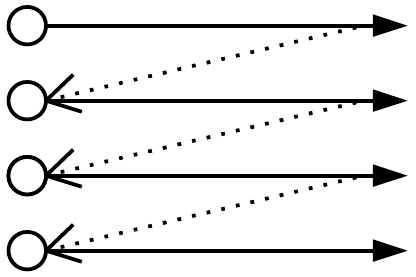
\includegraphics[scale=0.25]{pics/leftright.png}
      }
      \subfigure{
        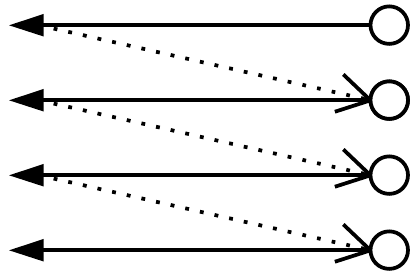
\includegraphics[scale=0.25]{pics/rightleft.png}
      }
      \subfigure{
        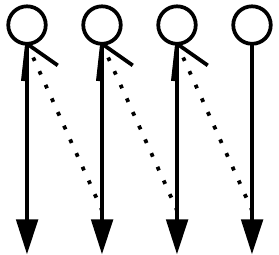
\includegraphics[scale=0.27]{pics/topbottom.png}
      }
      \caption{Writing orientation: 1) Horizontally Left-to right, 2) Horizontally Right-to-left 3) Vertically Right-to-left}
    \end{figure}

    As a result from this review of different human properties, there is need for making a narrowed selection of of the listed properties that looks promising to give any results in the analysis. As stated earlier, the goal of this research is not to prove that all human properties will impact users choice of patters, but make a selection of human properties that this study find promising to look further into. The human properties that will be included in the analysis is the  "reading/writing orientation", "hand size", "Left- or right-handed". Beside the the three main selected properties, I want to collect some demographics and other background information about the users and their mobile devices. This will further be described in Section~\ref{sec:datacollection}. We will now (Subsection~\ref{sec:scenario}) look further into the selected properties in hypothetical scenarios to provide further understanding of the selected properties and possible observations that may occur when analyzing the collected data. 

    \subsection{Sampling Frame and Technique} \label{sec:sampling}
      
      The survey type is categorized as ``non-probability sampling'' and the chosen sample technique is ``self-selection strategy''. This is chosen due to time and cost estimates, and the lack of control of respondents. A Purposive sampling technique would maybe provide a more uniformly collection of people, but it is hard to control respondents when the questionnaire is distributed on the Internet. The self-selection strategy will collect data from any respondents, and will be helpful when there is big population with potential respondents. The self-selection is a useful technique when we are not able to directly contact the potential respondents. When people select themselves for research, it might indicate that they have a strong feeling on the subject, or because they think it will bring them personal benefit or approval. 

      The target population for this research is in general all people with a mobile device. Because of the selected human properties and demographics, it is desirable to divide the target populations into subgroups. The subgroups can be used to control the responses during the data collection in order to provide a wide diversity in the data. 

      \todo{Legge til en liste med subgroups}

      We will now look further into some strategies for collecting data in Subsection~\ref{sec:response} from some of the subgroups that is outside my own network that might be harder get responses from.

    \subsection{Response Rate and Non-responses} \label{sec:response}

      When sending out the questionnaire I have no control over how many that are willing to respond, or how many people from different subgroups I am able to reach. To be able to reach the amount of data needed for a analysis, I need to look for a strategy that may increase the number of responses from the different subgroups. If I suspect that certain types of people in my sample are less willing to respond or harder to reach. I could deliberately include more of that subgroup in my sample so I can assure that I receive the number of respondents that I need. Maybe go face-to-face if a special group of people may be less willing to participate. 

      In this list there will be made a strategy for collecting data from the  different subgroups. {\it First}, some subgroups might be less willing to respond to the questionnaire. {\bf Second}, some of the subgroups might be harder to reach because they are outside of my own network. 

      \begin{itemize}
        \item {\bf People with age of 50 or higher:} People with the age over 50 may not own their own smartphone, or may be hard to reach for other reasons. I need to find networks were there is a high representation of people with a age of 50 or higher. In Norway there is a network called ``Seniorweb''. There is also a magazine called ``vi over 60'' that is a network that is highly represented with people with an age over 60. Both networks are possible to contact if there is a lack of respondents from this subgroup. 
        \item {\bf People with a different field of interest than IT and security:} My own network is overrepresented by people with a profession in IT and security. I need to be able to find other networks to be able to reach out to other people wither other professions. To reach out to people with other professions, it is a possibility to use the network from my family or directly contact a company. The university is a good start because of the high representation of different field of study. 
        \item {\bf People with a reading orientation from right-to-left:} The main reading orientation is from right-to-left, with a exception with some Arabic an Asian nationalities. My network do not include a high sample of people that have a other reading and writing orientation than my own. To reach out to other nationalities I can contact NTNU and ask for help to distribute my questionnaire to countries where NTNU have exchange programs. ``International section'' or other networks like ``ISFiT'' (International Student Festival in Trondheim). 
        \item {\bf People living in a different country than Norway:} I need to get in touch with people from different nationalities in order to get diversity in the collected data. I will contact the International Section at my university to ask them to distribute my questionnaire to the exchange students at my university. I am also having a trip to Minnesota in USA in the following spring, and I will use my time there recruiting people to respond to my questionnaire. During this semester I have been talking to researchers in other countries because of their interest in my research. Hopefully, they can provide help to distribute the questionnaire within their own networks. As stated earlier, ``ISFiT'' is the international student festival in Trondheim. There is people traveling from all around the world to Trondheim. 
        \item {\bf People that are left-handed:} There is a significant higher percentage of people that are right-handed, meaning that there is a possibility for getting more responses from people that are right-handed. Selecting a strategy for this is hard because there is not a known official network for left-handed people. There is a possibility for using groups at Facebook like ``Left-Hander's Club'' or the website called ``Left-handers day''. 
      \end{itemize}

      When analyzing the collected data, I need to find subgroups that have responded and those who have to responded. This will be used to make a discussion of why it lacked responses from a particular subgroup. The reason why this is important is because their non-response might be meaningful in its own right, or their lack of responses may have introduced bias in the data. This part is out of scope for this thesis, but need to be considered in the next phase of this research.
    
    \subsection{Sample Size} \label{sec:samplesize}

      I need to decide how big I want my final sample to be, taking into account my best estimate of the likely non-response rate of participants. When looking at my target population that is very wide. My target population is higher than 1 million, and therefore I would probably would need 1000 respondents or more.

      Because of the lack of control of the diversity of the respondents, there is likely to be some data properties that have a higher representation that others. Therefore it is important to control the data collected during the spring. If it occurs that a subpopulation is overrepresented, it is desired to use the strategy for smoothing the data from Subsection~\ref{sec:response}. The data collected should never be manipulated, and in a situation where there is lack of respondents from a subgroup, the only thing that I can do is to contact networks where there is a higher possibility to reached the subgroup that is underrepresented in the data.

      The total sample size is quite high, but should be manageable. If the total amount of 1000 respondents is not reached, a minimum number of respondents should be accepted at 500. In the analysis it will be hard to make any conclusions if the total number of respondents is too low.  The Internet offers researchers the possibility of accessing many people across the world cheaply and quickly. Not everyone have Internet access, and that need to be considered in the design.
